\pagestyle{plain}
\newpage{}
\qquad

\newpage{}
\section{Anexos}
\begin{instrucciones}
  El informe debe ir soportado por los anexos correspondientes a los que se hace alusión en los numerales 6 y 7 y en los cuadros 1 y 2, tales como:
* Copias de las publicaciones de resultados de conocimiento (en revistas científicas, libros o capítulos de libro) directamente relacionados con los objetivos del proyecto, o artículos en cualquier etapa del proceso de sometimiento a revistas científicas; 
* Copias de registros, patentes, normas o certificaciones de que éstas están en proceso de solicitud o evaluación;
* Copias de certificaciones de la existencia y calidad de productos o procesos tecnológicos obtenidos como resultado del proyecto;
* Copias de los resúmenes de las ponencias presentadas en eventos científicos;
* Copias de otro material divulgativo que se haya producido sobre los resultados de la investigación;
* Resúmenes de las tesis o trabajos de grado que se hayan desarrollado en el marco del proyecto;
* Cualquier otro material que soporte los resultados obtenidos.
\end{instrucciones}



\subsection{Artículos científicos}
\label{sec:artic-cient}

%\subsubsection{DOI: 10.1103/PhysRevD.97.115032~\cite{Reig:2018mdk}} 
%\label{sec:physr1}

%\newpage


%\begin{includepdfs}%10.1103
%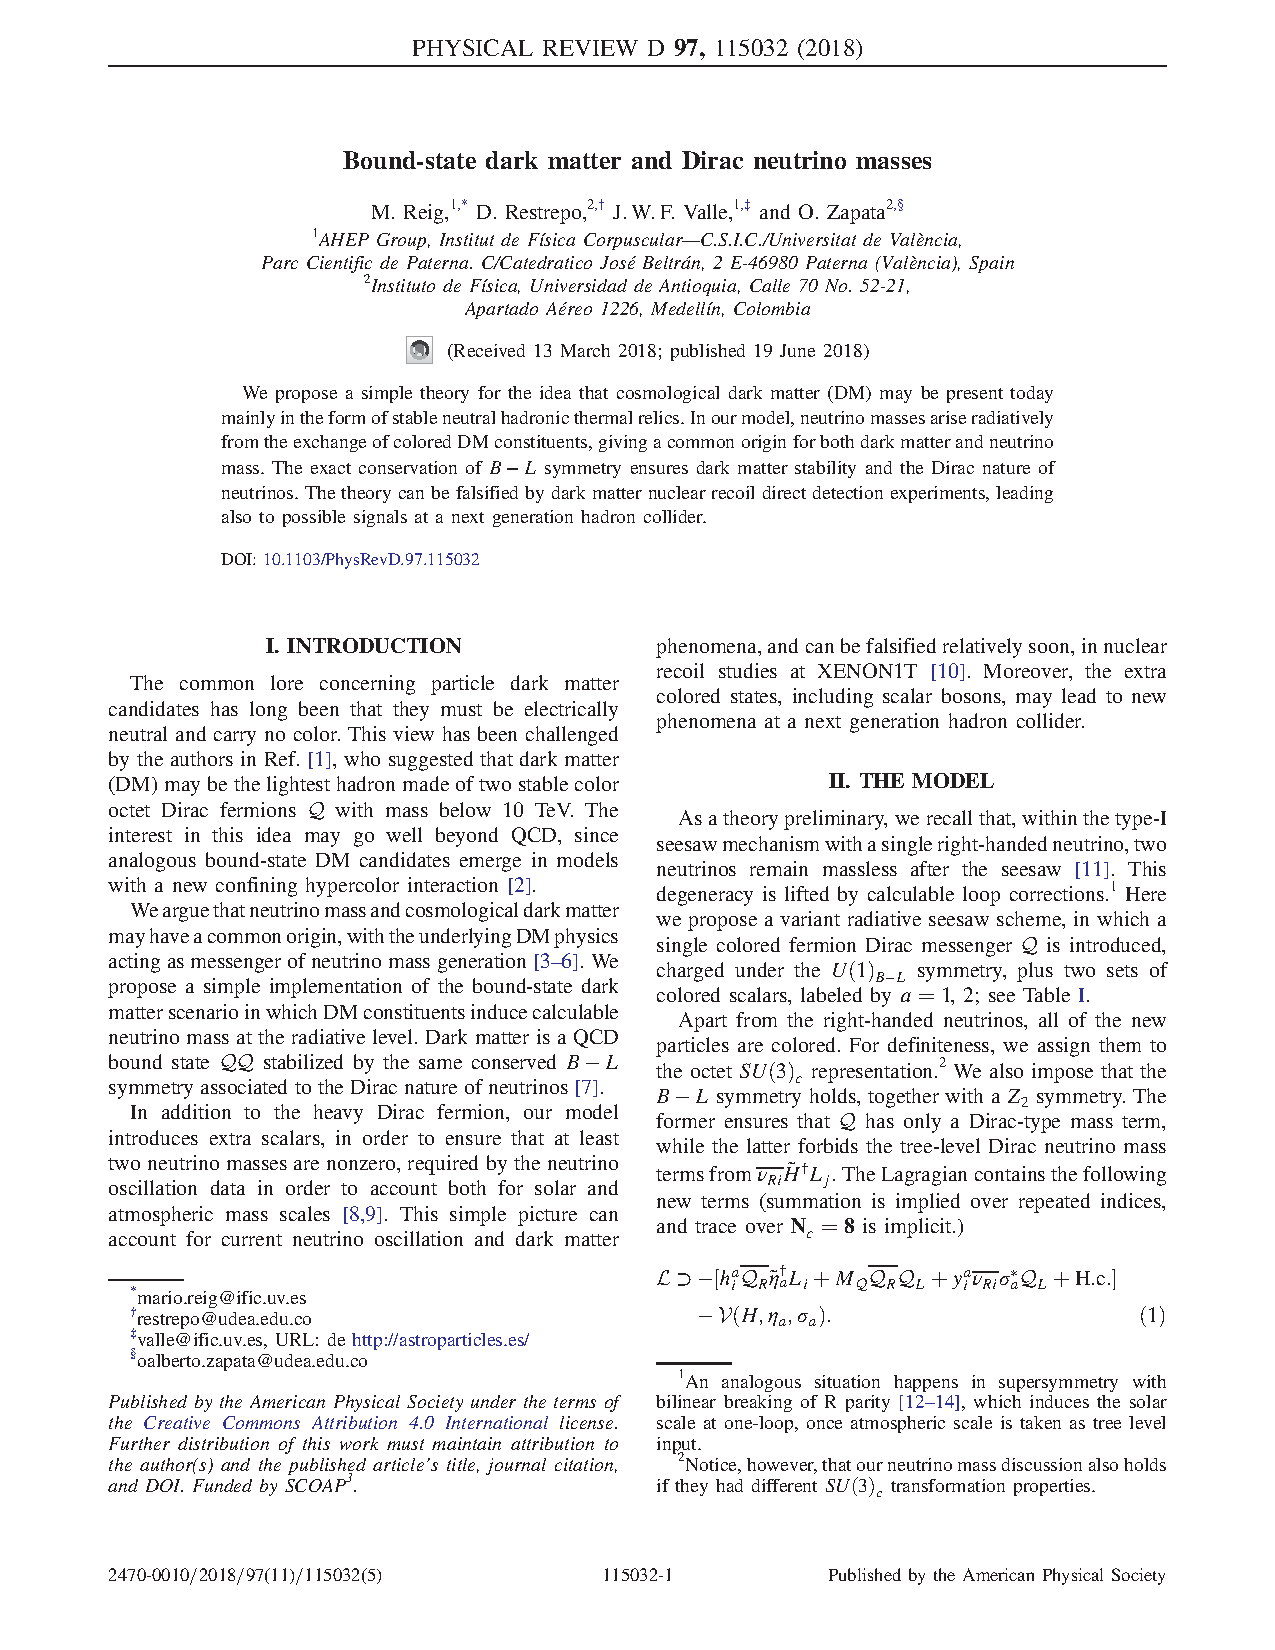
\includepdf[pages=-]{articles/PhysRevD-97-115032.pdf}  
%\end{includepdfs}

%\newpage{}


          


%%% Local Variables: 
%%% mode: latex
%%% TeX-master: "informefinal"
%%% ispell-local-dictionary: "castellano8"
%%% End: 
